\chapter{Introduction}

Data is now at the center of organizations. 
Data is heterogeneous, meaning that there is an explosion of Data Sources that each exposes data in its own format 
that be structured, semi-structured or non-structured.
Data needs to be real-time, because organizations no longer want to wait a day to have reports and alerts on their business data.
Data needs to be resilient and logged: all changes in the data should be stored and queryable for future system audits.
\\

To achieve these requirements, traditional monolithic Data Wharehouse software start to be out-dated. They often
propose to deal with only structured data to map it in a relational model, and are often batch-oriented: 
the ETL mechanism (data extraction, transform and load) regularly happen once or twice day, and there is no mechanism 
for real-time subscriptions of new events happening on the data \footfullcite{bib:linkedinLog}.
\\

The platform I present in this thesis is an event-oriented Data Integration and Stream Processing platform that allows data consumers
to subscribe to data changes in real-time. The main shift from traditional data wharehouse software is that the whole
system is organized around the notion of \textit{event} (\textit{log}). Data Sources emit events that represents the changes 
of the data, not the current state of the data. Based on the Event-Sourcing principle \footfullcite{bib:eventSourcing}, events
are stored in a Journal that is a sequence of immutable changes to the data. Then, the stream of events coming from the Journal 
can be processed by data consumers that can react to the change of data. An example of data consumer can be one that maintain
a pre-computed view on the data that is updated upon each event, or one that push notification to another service upon a certain
kind of events (see Figure \ref{fig:main_archi} for the global architecture).
\\

An example use case is when an organization uses different SaaS services for each of its teams. For instance, the sales
team use a SaaS software to process their sales pipeline, the project management team use another SaaS software to manage
the production teams, etc... Without a central data backbone, it is not possible to have a global view on the company data.
The platform I present in this thesis can integrate these different SaaS softwares using their REST API, detect what
changes have been made on the data, and emits the corresponding events. As a result, data consumers can use these events
to update in real-time dashboards about the company data, mixing the data coming from different sources. A data consumer can also push a
notification to SaaS service X when it receives an event from SaaS service Y, allowing real-time synchronization between
data sources.
\\

An advantage of Event Sourcing is that the whole history of the system is stored. Events are immutable changes made to the data
and are always append to the Journal (never deleted or modified). As a result, the system stores not only the current state
of the data, but also all its previous states. This allows two interesting properties.

First, Queries on data history:

Second, fault-tolerance and re-playability:
\\ 

This approach is also known as CQRS \footfullcite{bib:cqrs}. The core principle of CQRS is to decouple the write part and read part
of a system. The write part (Data Integration) only need to push immutable events to the Journal in an append-only fashion, which
is very efficient because there is no mutation of the data and no read-write contentions as in traditional databases.
The read part is a set of denormalized pre-computed view that are optimized for low read latency (as the view are automatically re-computed
when a new related event comes in). 
An obvious property that causes this architecture is eventual consistency: when a data producer has received the acknowledgment
from the Journal, there is no guarantee that data consumers has already processed the event and updated the data view.

This model also allows very easy distribution and heterogeneity of the platform. Easy distribution because it is a message-oriented
architecture where each component (data producer, journal, data consumers with data views) only exchange message (events) to each other with
no shared-state. This comes with the possibility of using heterogeneous technologies because parts are decoupled and only needs
to communicate via defined protocols.
\\



The platform consists of three main parts: 
\begin{itemize}
  \item Data Integration, that must integrate several data sources in order to emit 
events (data changes) to the Journal. 
  \item Journal, an abstraction for a sequence of immutable events. The Journal must expose methods to insert events,
  and expose methods to subscribe to the stream of events.
  \item Stream processing, where one can define a tree of data consumers (stream processors) that can react to
  events, maintain derived pre-computed view of the data, and emit new stream of events.
\end{itemize}

\begin{figure}[h]
  \begin{center}
    \makebox[\textwidth]{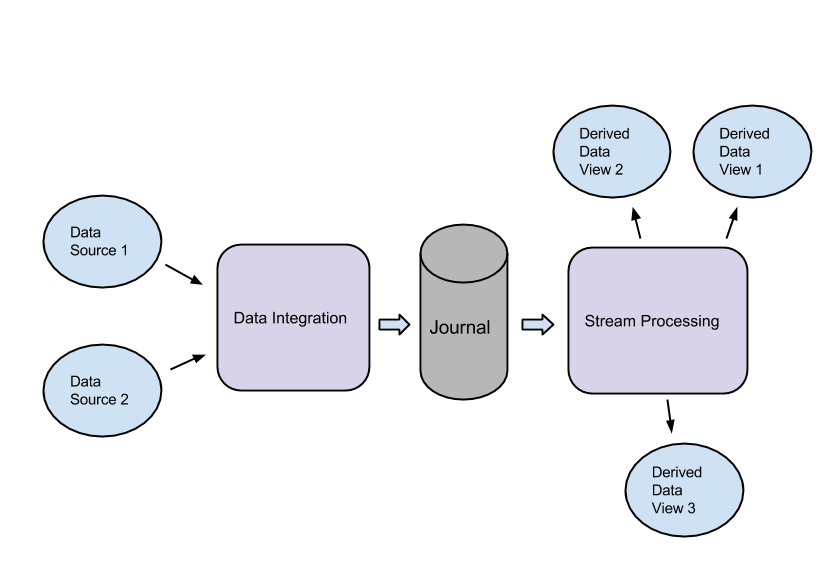
\includegraphics[width=1.0\textwidth]{img/main_archi.png}}
    \caption{Global architecture}
    \label{fig:main_archi}
  \end{center}
\end{figure}

Nonetheless, this kind of evented architecture must be done with a lot of care concerning technical architecture.
The platform needs to do lot of IO in order to push the stream of events from data sources to data consumers, and must
parallelize a lot of operations. Moreover, it must ensure that the stream of events (producer) does not overwhelmed the stream
processors (consumers), i.e if consumers process data slowly, producer must try to slow the push rate. It should also deal with possible
failure of components and offer strong guarantees on these cases (like no message loss).

In order to fulfill those requirements, an asynchronous non-blocking approach will be taken to develop the platform in order to
minimize IO cost, decouple components to be able to distribute them easily, take easily advantage of parallelization and handle failure based on the 
Reactive Programming manifesto principles \footfullcite{bib:reactiveManifesto}. The platform is developed using functional programming in
the Scala programming language \footfullcite{bib:scala} in order to use function abstractions to better handle asynchronous and stream-oriented code.
\\

This report is divided into two main parts: the Data Integration part, and the Journal and Stream Processing part.
In each part, I describe the functional and non-functional requirements of the components, and then I present the technical architecture
and implementation.

